\documentclass[tikz,border=2pt]{standalone}
\usepackage{amsmath,amssymb}
\usepackage{tikz}

\begin{document}
% Disjoint (mutually exclusive) events cannot both happen: no overlap, so probabilities add.
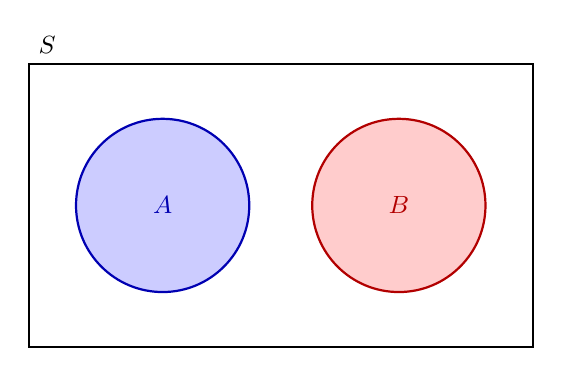
\begin{tikzpicture}[every node/.style={font=\small}]
	\draw[thick] (-3.2,-1.8) rectangle (3.2,1.8);
	\node[anchor=south west] at (-3.2,1.8) {$S$};
	\fill[blue!20] (-1.5,0) circle (1.1);
	\fill[red!20] (1.5,0) circle (1.1);
	\draw[thick, blue!70!black] (-1.5,0) circle (1.1);
	\draw[thick, red!70!black] (1.5,0) circle (1.1);
	\node[blue!70!black] at (-1.5,0) {$A$};
	\node[red!70!black] at (1.5,0) {$B$};
	
\end{tikzpicture}
\end{document}
